%% LaTeX-Beamer template for KIT design
%% by Erik Burger, Christian Hammer
%% title picture by Klaus Krogmann
%%
%% version 2.1
%%
%% mostly compatible to KIT corporate design v2.0
%% http://intranet.kit.edu/gestaltungsrichtlinien.php
%%
%% Problems, bugs and comments to
%% burger@kit.edu

\documentclass[18pt]{beamer}

%% SLIDE FORMAT

% use 'beamerthemekit' for standard 4:3 ratio
% for widescreen slides (16:9), use 'beamerthemekitwide'

\usepackage{templates/beamerthemekit}
\usepackage[utf8]{inputenc}
\usepackage{pdfpages}
% \usepackage{templates/beamerthemekitwide}

%% TITLE PICTURE

% if a custom picture is to be used on the title page, copy it into the 'logos'
% directory, in the line below, replace 'mypicture' with the 
% filename (without extension) and uncomment the following line
% (picture proportions: 63 : 20 for standard, 169 : 40 for wide
% *.eps format if you use latex+dvips+ps2pdf, 
% *.jpg/*.png/*.pdf if you use pdflatex)

\titleimage{schloss}

%% TITLE LOGO

% for a custom logo on the front page, copy your file into the 'logos'
% directory, insert the filename in the line below and uncomment it

\titlelogo{algoLogo}

% (*.eps format if you use latex+dvips+ps2pdf,
% *.jpg/*.png/*.pdf if you use pdflatex)

%% TikZ INTEGRATION

% use these packages for PCM symbols and UML classes
% \usepackage{templates/tikzkit}
% \usepackage{templates/tikzuml}

% the presentation starts here

\title[Distributed Node Coloring for Directed Graphs]{Distributed Node Coloring for Directed Graphs}
\subtitle{Bachelorarbeit, Betreuer: Fabian Fuchs, Roman Prutkin}
\author{Manuel Schweigert}

\institute{Institut für Theoretische Informatik}

% Bibliography

\usepackage[citestyle=authoryear,bibstyle=numeric,hyperref,backend=bibtex]{biblatex}
\usepackage{csquotes}
\addbibresource{templates/example.bib}
\bibhang1em

\setbeamerfont{caption}{size=\footnotesize}

\begin{document}

% change the following line to "ngerman" for German style date and logos
\selectlanguage{ngerman}

%title page
\begin{frame}
\titlepage
\end{frame}

\section{Einführung}
\begin{frame}{Einführung}
\begin{tabular}{l l}
\begin{minipage}{0.5\textwidth}
	\begin{itemize}
		\item Knotenfärbung klassisch
		\item Verteilte Knotenfärbung
		\item Kommunikationsmodelle (SINR, Congest)
	\end{itemize}
\end{minipage}
&
\begin{minipage}{0.45\textwidth}
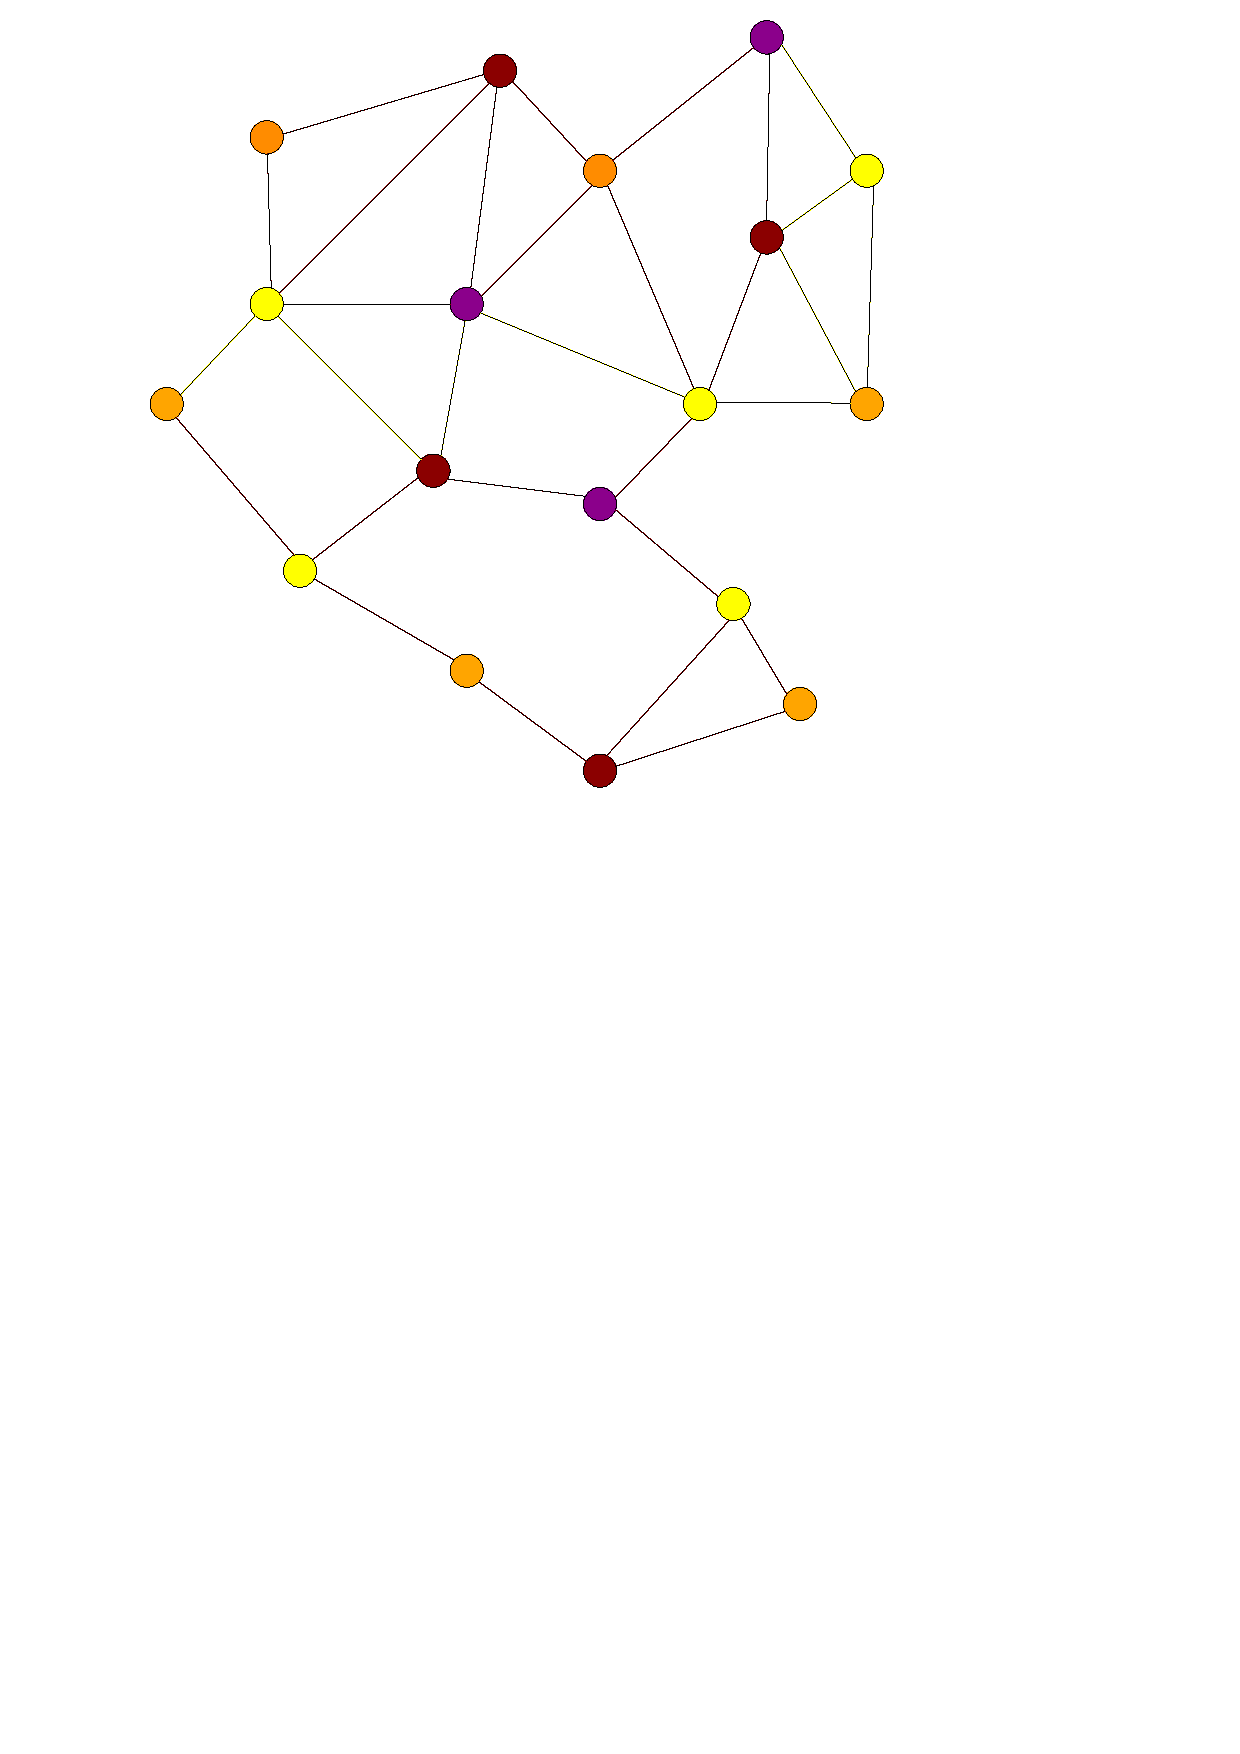
\includegraphics[width=\textwidth]{pdf/nodecoloring.pdf}
\end{minipage}
\end{tabular}
\end{frame}

\begin{frame}{Motivation}
\begin{tabular}{l l}
\begin{minipage}{0.5\textwidth}
   \begin{exampleblock}{Kommunikationsgraph}
     \begin{itemize}
			 \item<1-> Knoten mit Sendereichweite
			 \item<2-> Bisher immer uniform
			 \item<3-> Resultiert in einem ungerichteten Kommunikationsgraph
			 \item<4-> Szenario: verschieden starke Sendeleistung
			 \item<5-> Resultat: gerichteter Kommunikationsgraph
		 \end{itemize}
   \end{exampleblock}
\end{minipage}
&
\begin{minipage}{0.5\textwidth}
\includegraphics<1>[height=150pt, page=1]{pdf/commgraph.pdf}
\includegraphics<2>[height=150pt, page=2]{pdf/commgraph.pdf}
\includegraphics<3>[height=150pt, page=3]{pdf/commgraph.pdf}
\includegraphics<4>[height=150pt, page=4]{pdf/commgraph.pdf}
\includegraphics<5>[height=150pt, page=5]{pdf/commgraph.pdf}
\end{minipage}
\end{tabular}



\end{frame}

\begin{frame}{Gliederung}
\tableofcontents
\end{frame}
\section{Definitionen}
\begin{frame}{Definitionen}
\begin{tabular}{l l}
\begin{minipage}{0.5\textwidth}
	\begin{itemize}
		\item $\Delta$: maximaler Eingangsgrad
		\item valide Knoten-Färbung im gerichteten Graph: Nachbarn eingehender Kanten haben andere Farbe als Knoten
	\end{itemize}
\end{minipage}
&
\begin{minipage}{0.5\textwidth}
	
	\begin{center}
		\includegraphics[width=0.90\textwidth, page=2]{pdf/nodecoloring.pdf}
	\end{center}
\end{minipage}
\end{tabular}
\end{frame}

\begin{frame}
\begin{itemize}
		\item $D_v$ von $v$: Menge der Knoten $u$, sodass $\exists$ Kante mit $(u,v)\in E$ aber $(v,u)\notin E$
		\item $l$: Länge des längsten dominierenden Pfades im Graph
\end{itemize}
\begin{figure}
	\centering
		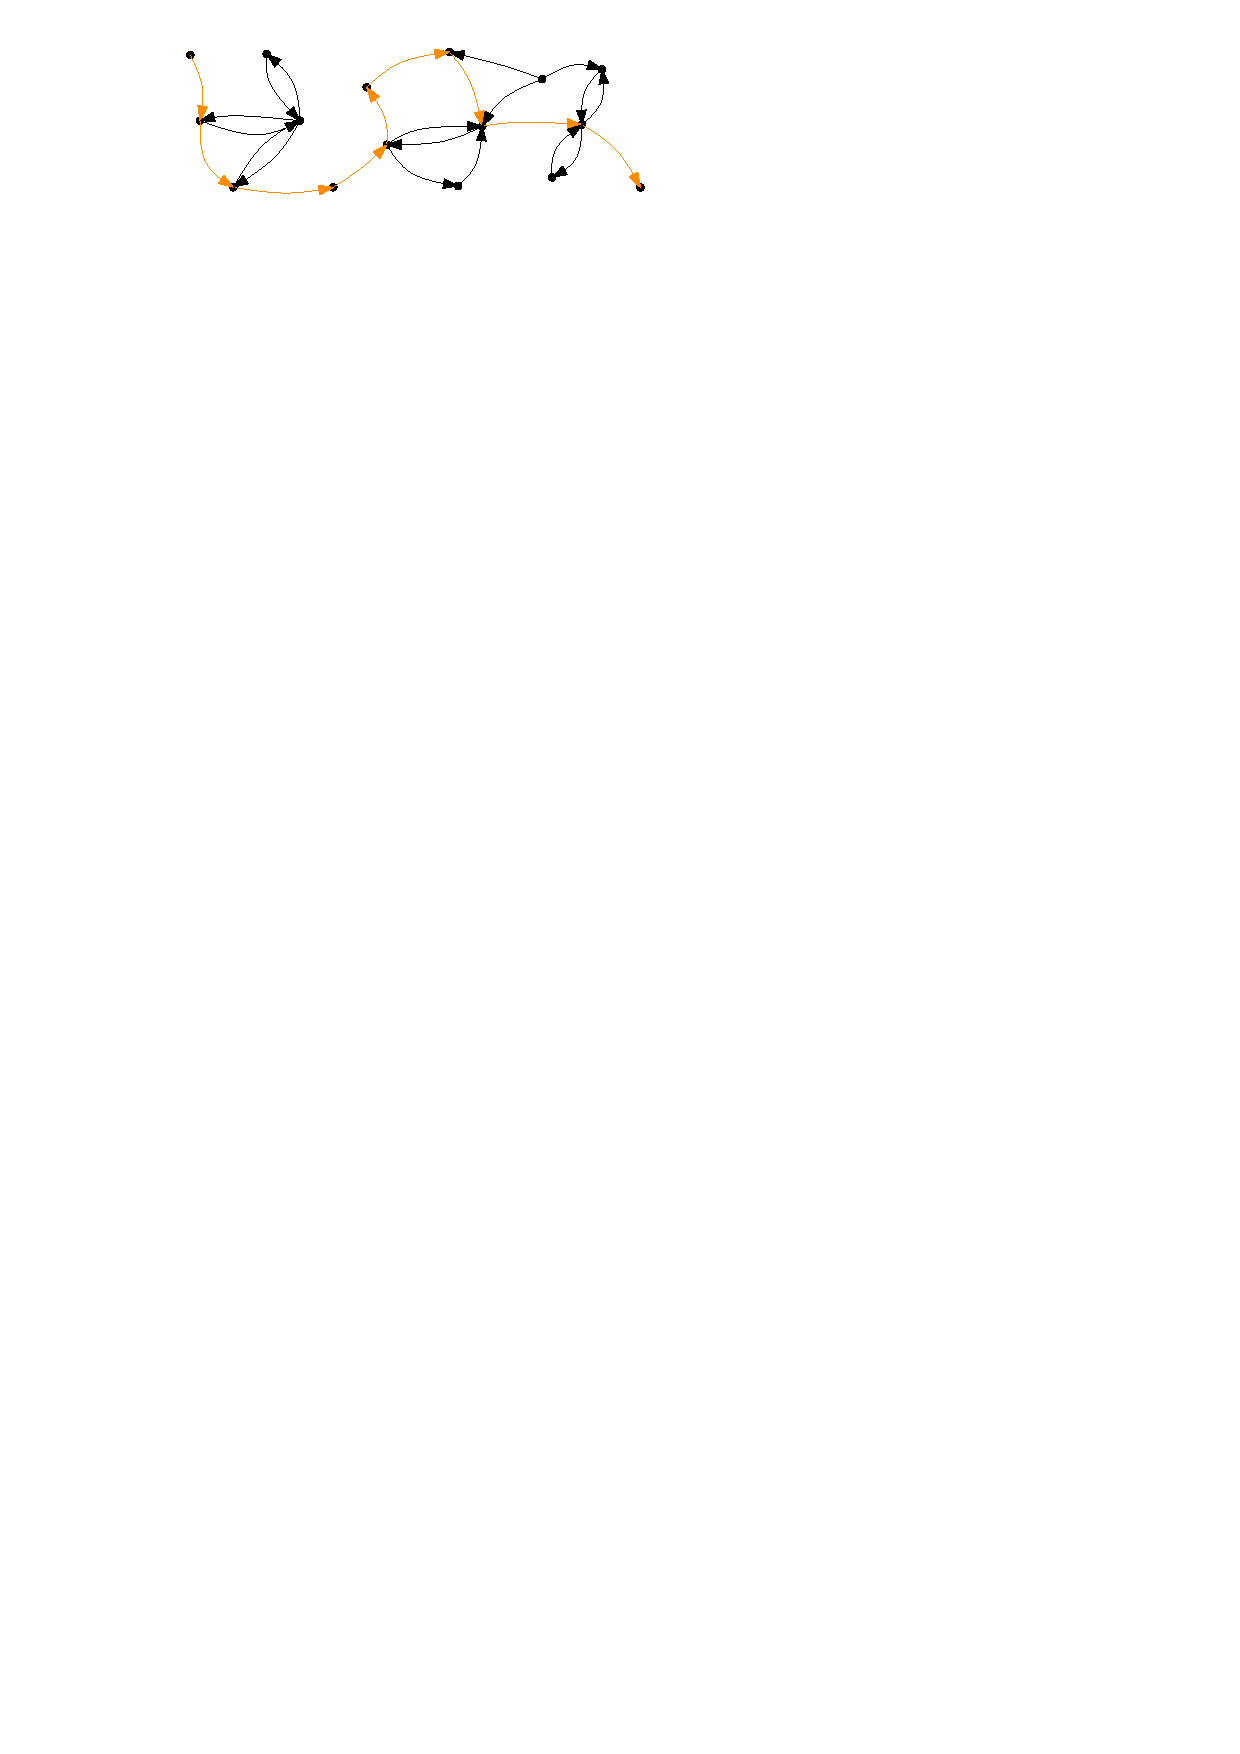
\includegraphics[width=0.90\textwidth,clip=true,trim=2cm 0pt 0pt 0pt]{pdf/longestpath.pdf}
	\label{fig:longestpath}
\end{figure}

\end{frame}


\section{Algorithmen}

\begin{frame}{Randomisierter Färbealgorithmus}
Grundidee:
\begin{itemize}[<+->]
	\item In jeder Runde:
	\item Jeder Knoten wählt sich zufällig eine Farbe
	\item Wenn konfliktfrei $\Rightarrow$ "`reserviere"' Farbe und terminiere
	\item Nachbarknoten respektieren reservierte Farben in der Zukunft
\end{itemize}
\end{frame}


\subsection{Mit Initialisierung}
\begin{frame}{Algorithmus Rand-Delta-Plus1}
	\begin{exampleblock}{Skizze}
	  \begin{itemize}
			\item Finde dominierende Knoten ($D_v$)
			\pause
			\item Hauptschleife
			\pause
			\begin{itemize}
				\item Mit Wahrscheinlichkeit $1/2$ setze aus
			\pause
				\item Wähle zufällige Farbe von $\Delta+1$ Farben
			\pause
				\item Broadcaste die Farbe an alle Nachbarn
			\pause
				\item Wenn kein Nachbar die gleiche Farbe hat und alle Knoten in $D_v$ fertig sind
				\begin{itemize}
					\item sende die gewählte Farbe als finale Farbe und terminiere
				\end{itemize}
			\end{itemize}
		\end{itemize}
	\end{exampleblock}
\end{frame}

\begin{frame}{Beweisskizze}
Subgraph-Hierarchie:
\only<1>{
\begin{figure}
\centering
		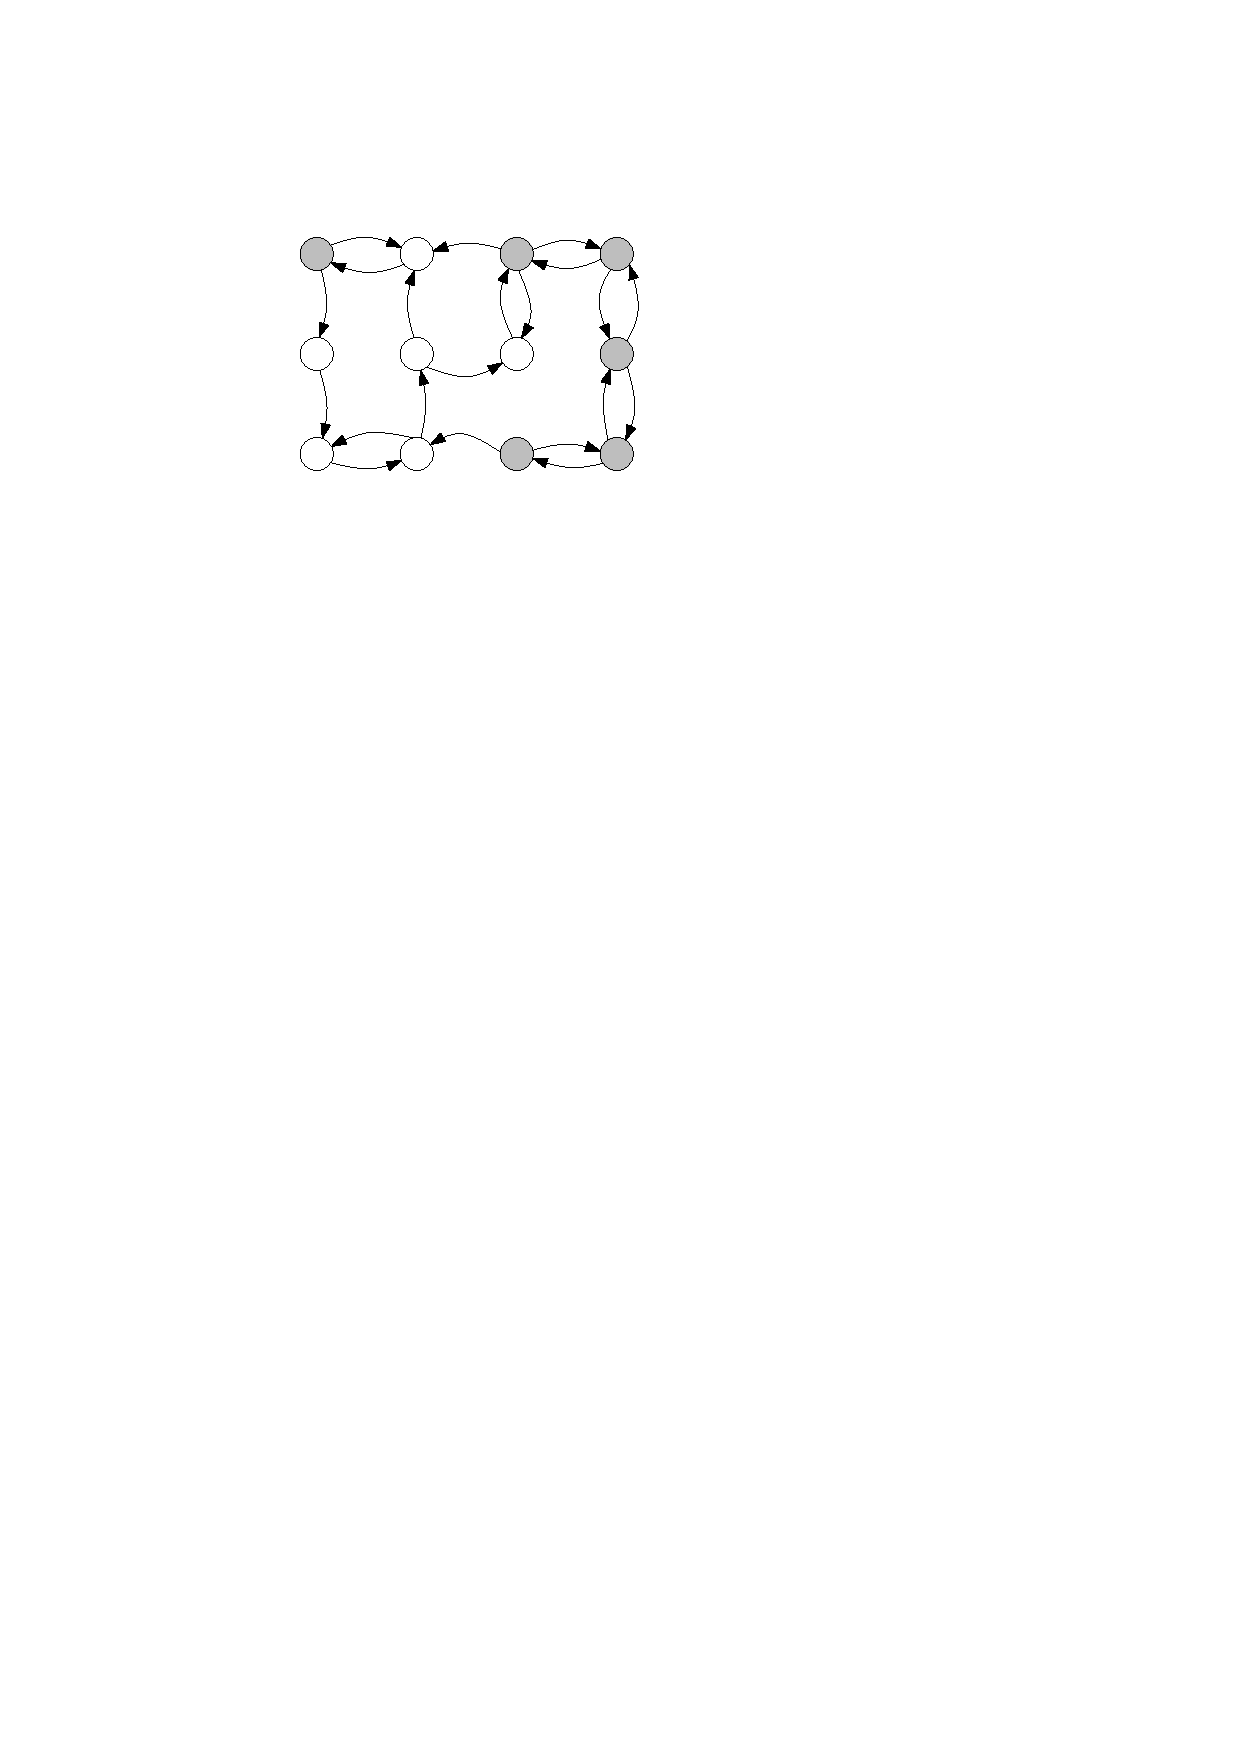
\includegraphics{pdf/G_1.pdf}
	\caption{Subgraph $G_1$, alle nicht-dominierten Knoten}
	\end{figure}
	}
	
\only<2>{
\begin{figure}
\centering
		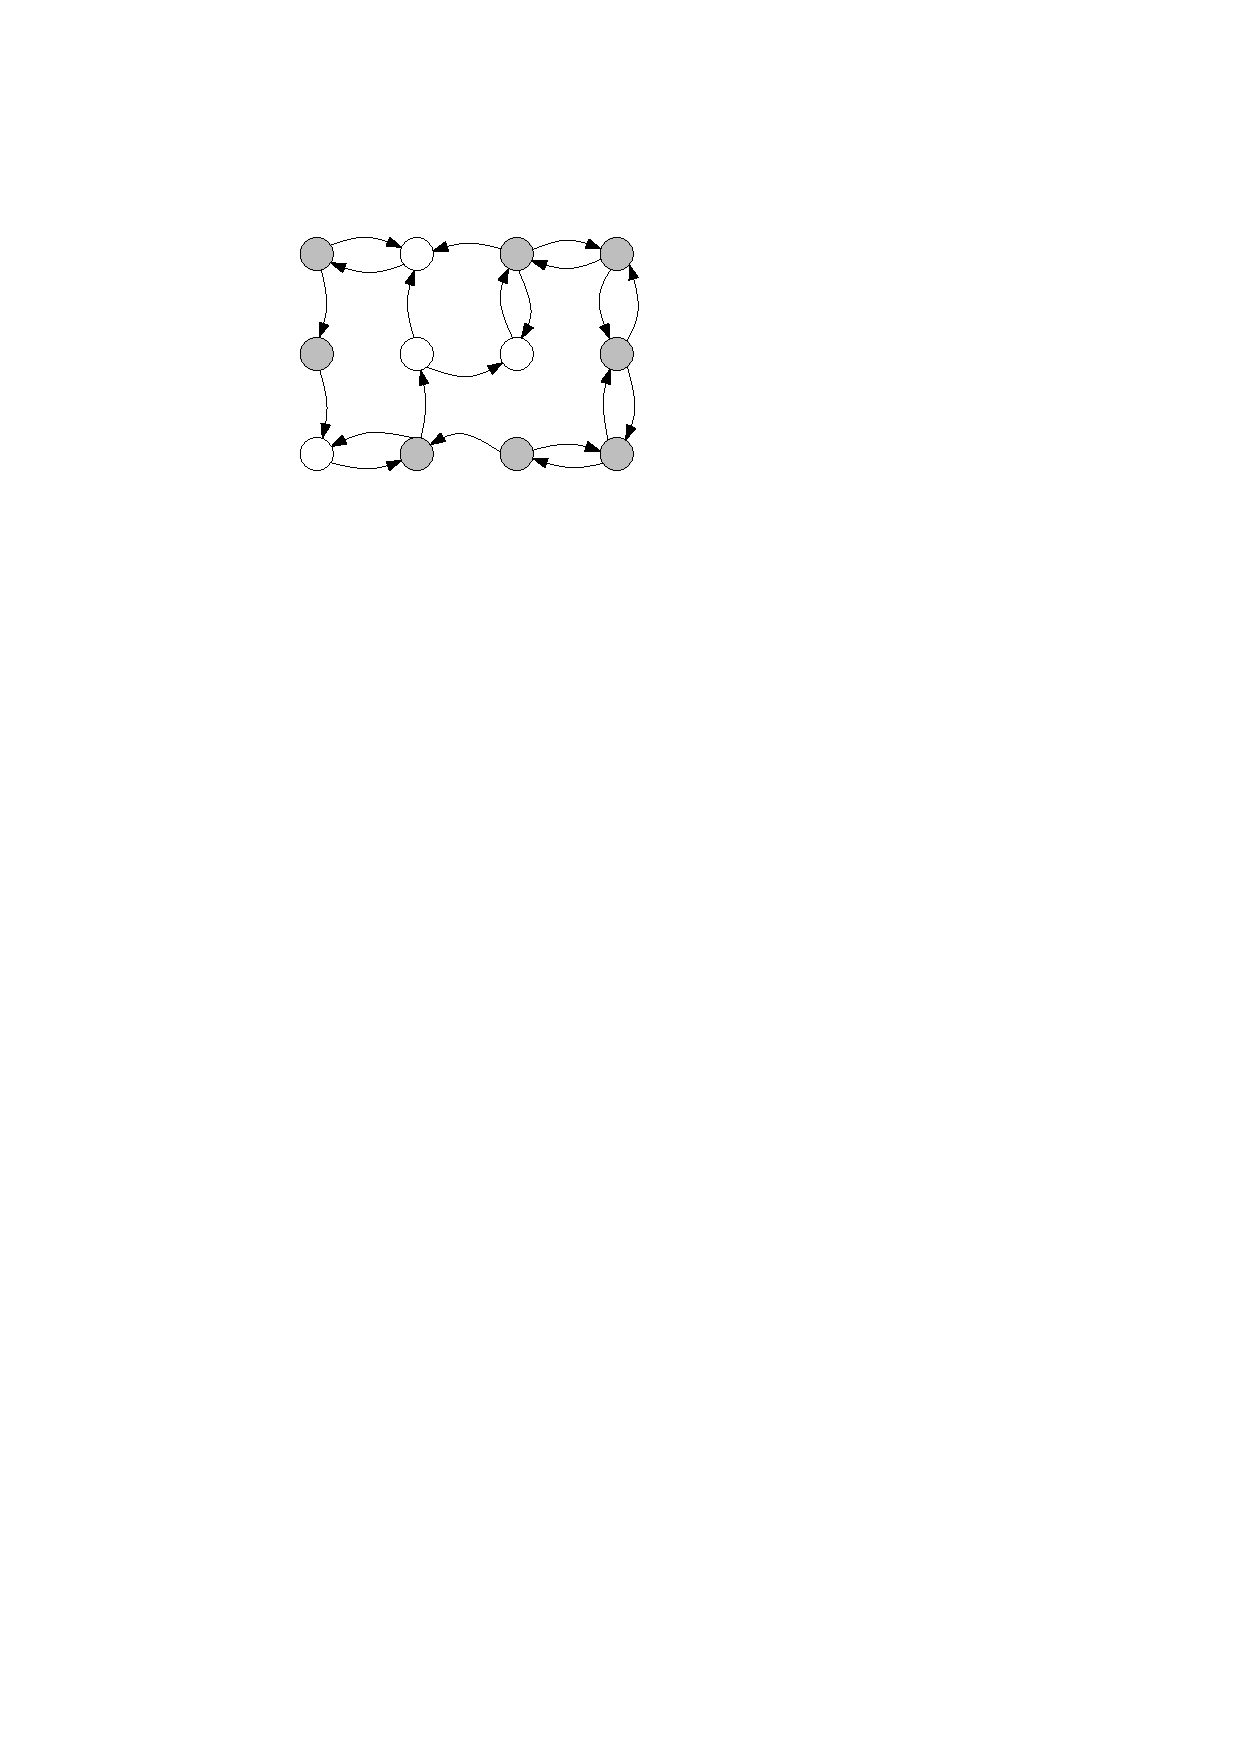
\includegraphics{pdf/G_2.pdf}
	\caption{Subgraph $G_2$, alle Knoten, die nur aus Knoten aus $G_1$ dominiert werden}
	\end{figure}
	}
	
\only<3>{
\begin{figure}
\centering
		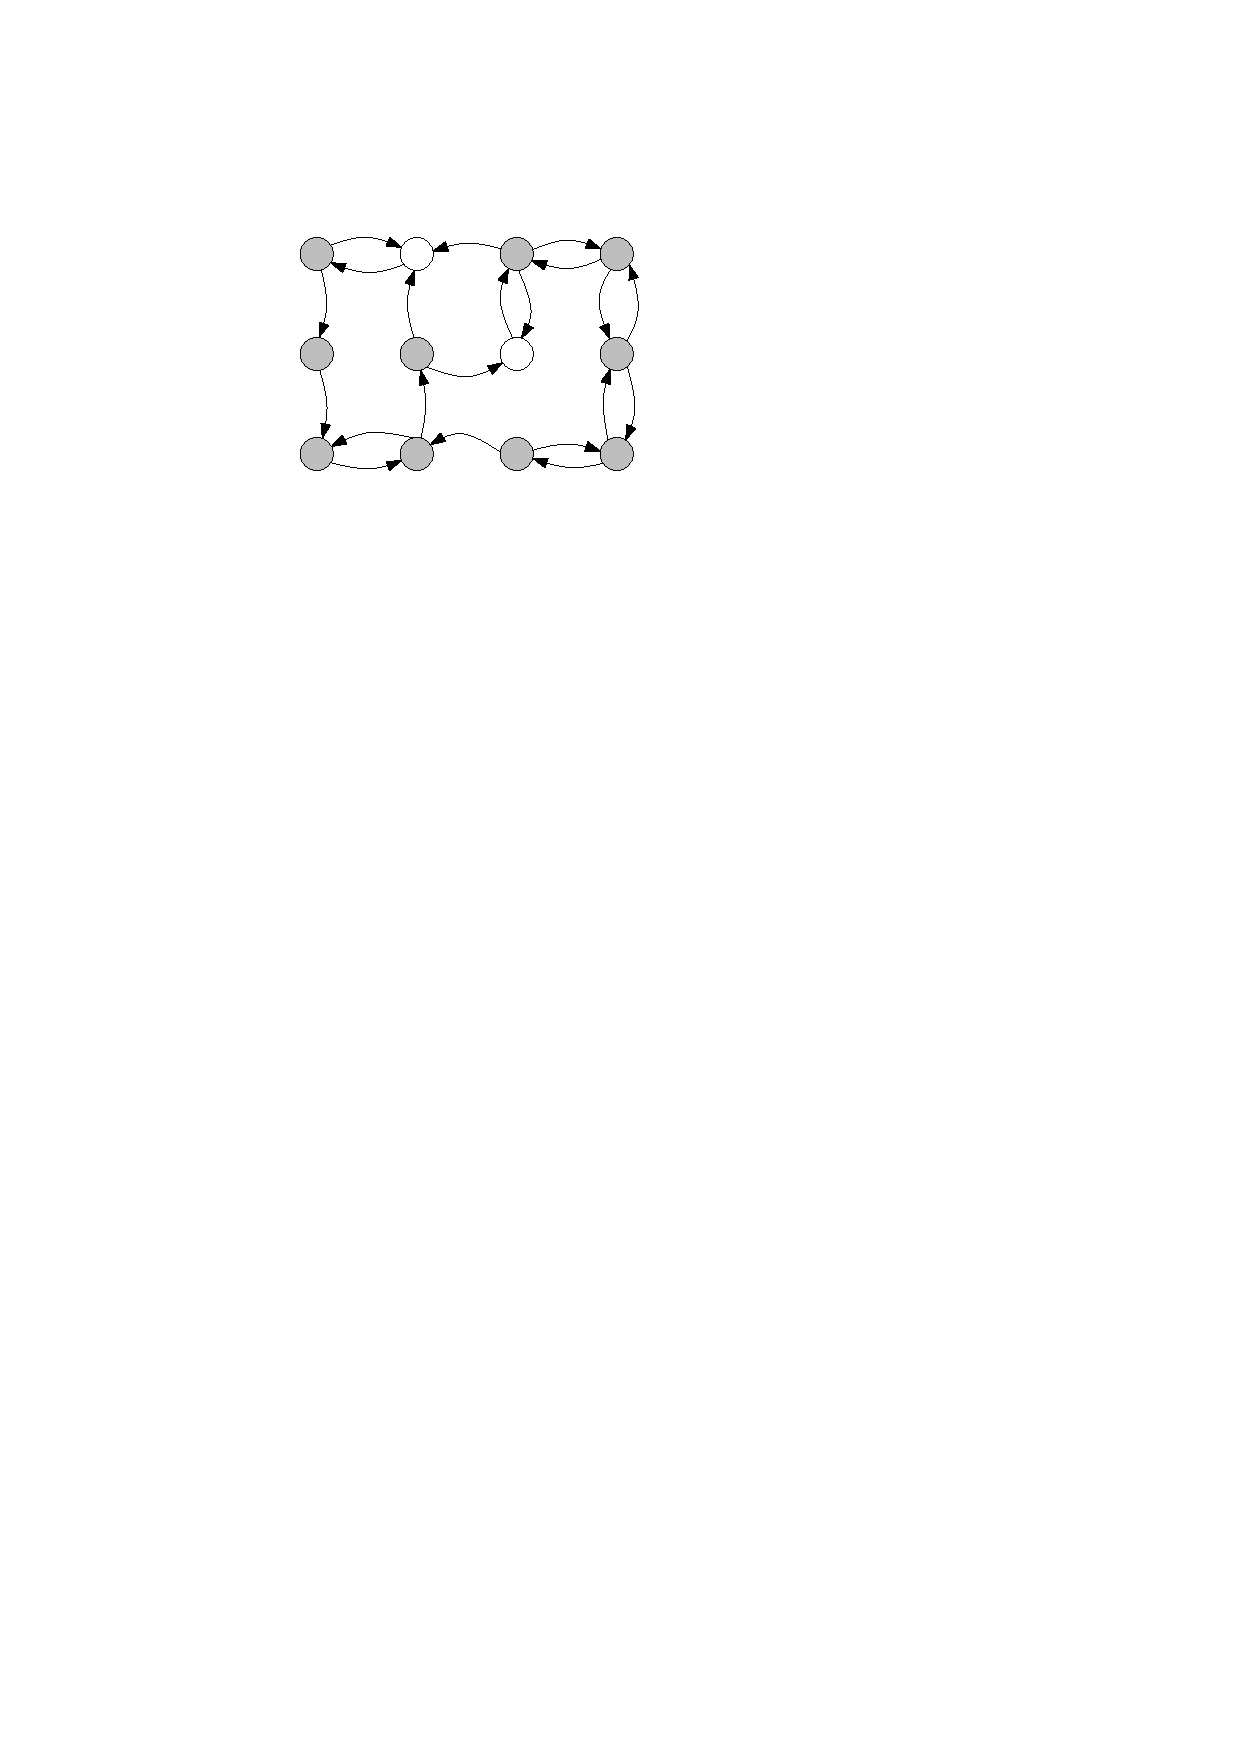
\includegraphics{pdf/G_3.pdf}
	\caption{Subgraph $G_3$, alle Knoten, die nur aus Knoten aus $G_2$ dominiert werden}
	\end{figure}
	}
	
\only<4>{
\begin{figure}
\centering
		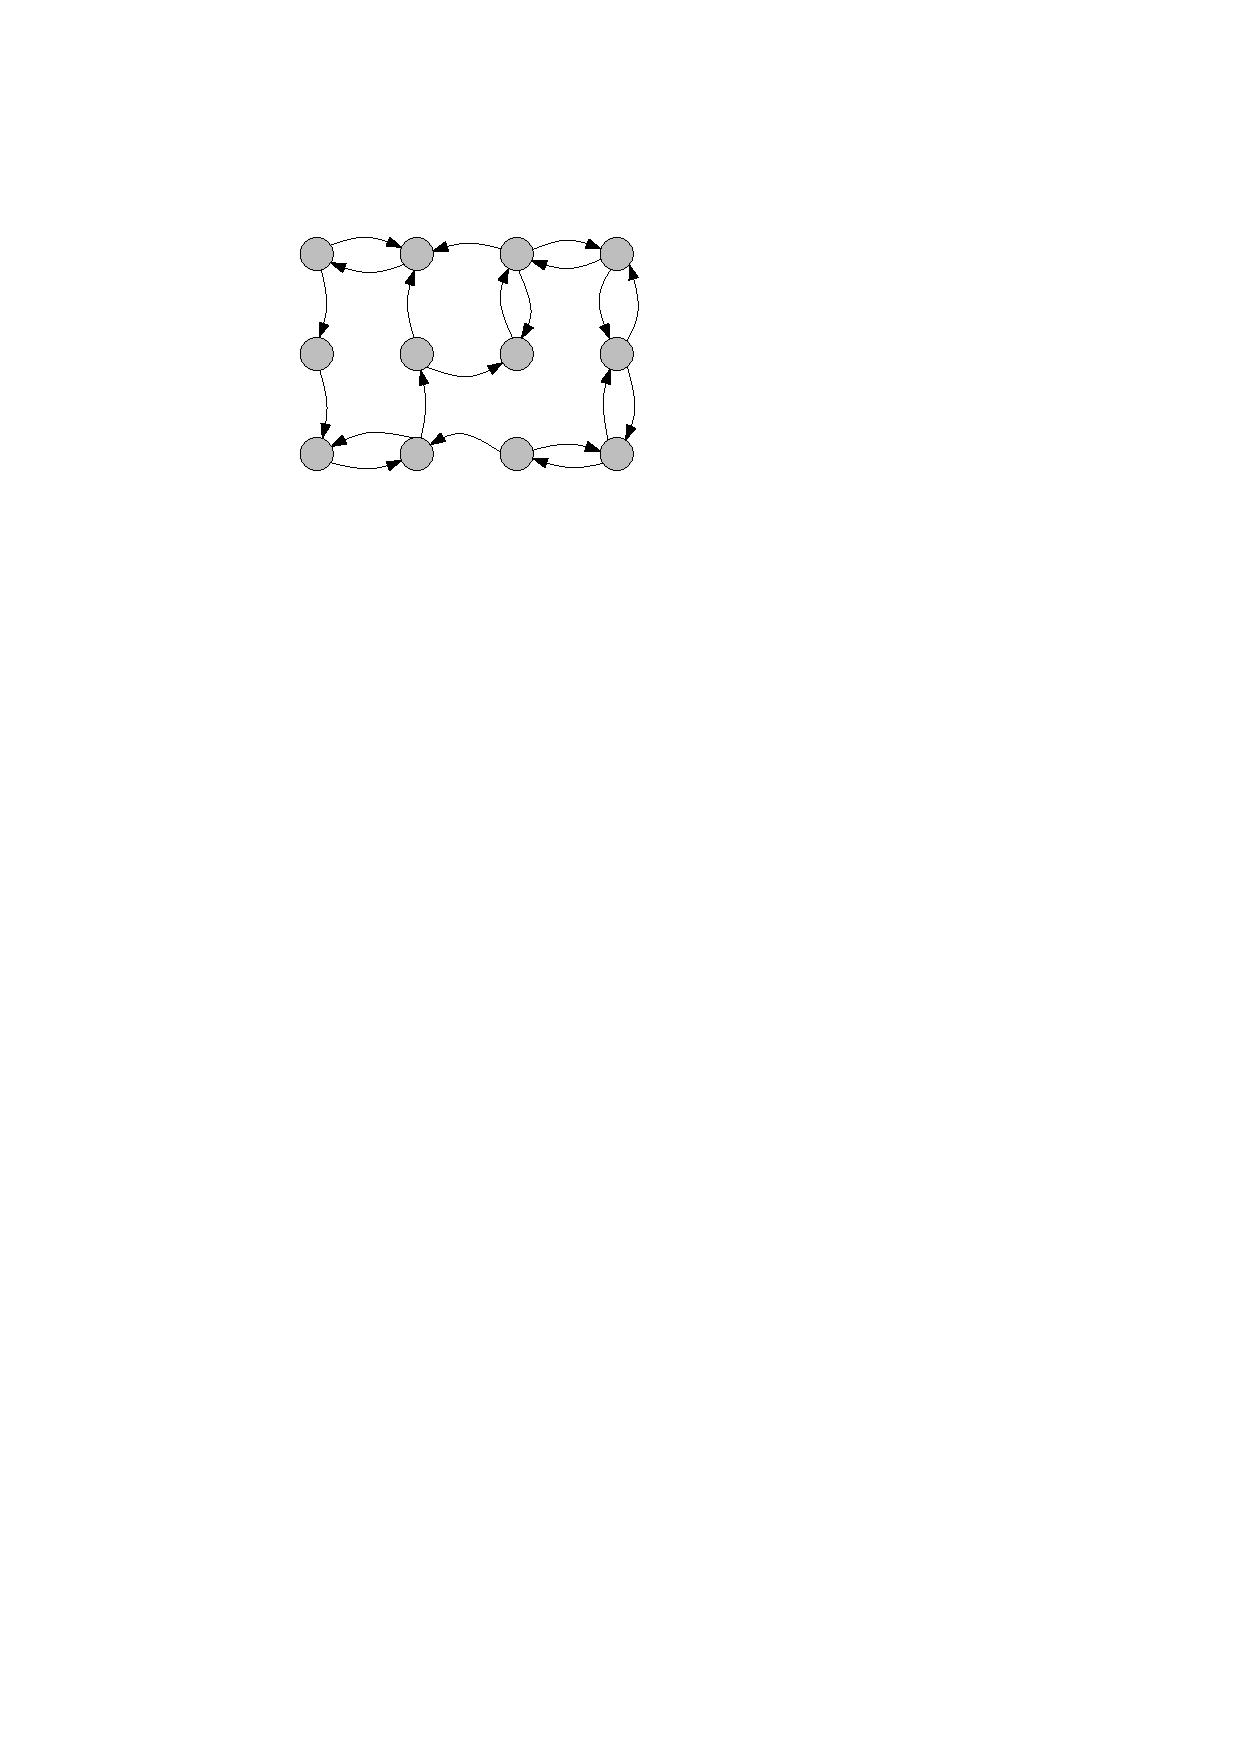
\includegraphics{pdf/G_4.pdf}
	\caption{Subgraph $G_4 = G$, alle Knoten, die nur aus Knoten aus $G_3$ dominiert werden}
	\end{figure}
	}

\end{frame}



\begin{frame}{Beweisskizze}
		\begin{itemize}
			\item Subgraph-Hierarchie
			\item Finde kleinstes $l$ sodass $G_{l+1} = G$
			\pause
			\item Zeige induktiv, dass Färbung von $G_k$ $\rightarrow$ $G_{k+1}$ max. $O(\log n)$ benötigt (mit hoher Wahrscheinlichkeit)
			\pause
			\item Laufzeit setzt sich aus Initialisierung ($O(\Delta)$) und $(l+1) \cdot O(\log n)$ zusammen
			\pause
		\end{itemize}
	$\Rightarrow$ Laufzeit ~$O(\Delta + l \log n)$
\end{frame}

\begin{frame}{Induktionsschritt}
		\begin{itemize}[<+->]
			\item Betrachte Knoten $v \in G_{k+1}$, der in der letzten Runde in einem Konflikt war und Münzwurf gewinnt
			\item Wahrscheinlichkeit für $v$ wieder im Konflikt ist $\leq (\Delta + 1  - |F_v|) \frac{1}{2 (\Delta + 1 - |F_v|)} = \frac{1}{2}$
			\item $\Rightarrow v$ terminiert mit Wahrscheinlichkeit $\geq (1/2 \cdot 1/2) = 1/4$
			\item In Runde $i$ hat $v$ mit Wahrscheinlichkeit $\leq (1-1/4)^i$ nicht terminiert
			\item $\Rightarrow$ Nach $(c+1) 4\log n$ Runden hat $v$ mit Wahrscheinlichkeit $\leq 1-1/n^c$ nicht terminiert
		\end{itemize}
\end{frame}

\subsection{Ohne Initialisierung}
\begin{frame}{Überlegung}
	\begin{itemize}[<+->]
		\item Initialisierung beansprucht $O(\Delta)$ Broadcasts
		\item Versuch: Algorithmus ohne Initialisierung
		\item Problem: Knoten kann sich nicht mehr sicher sein, ob er fertig ist oder nicht
		\item Resultat: Nachbarn respektieren und Farben halten
	\end{itemize}
	\uncover<3->{
	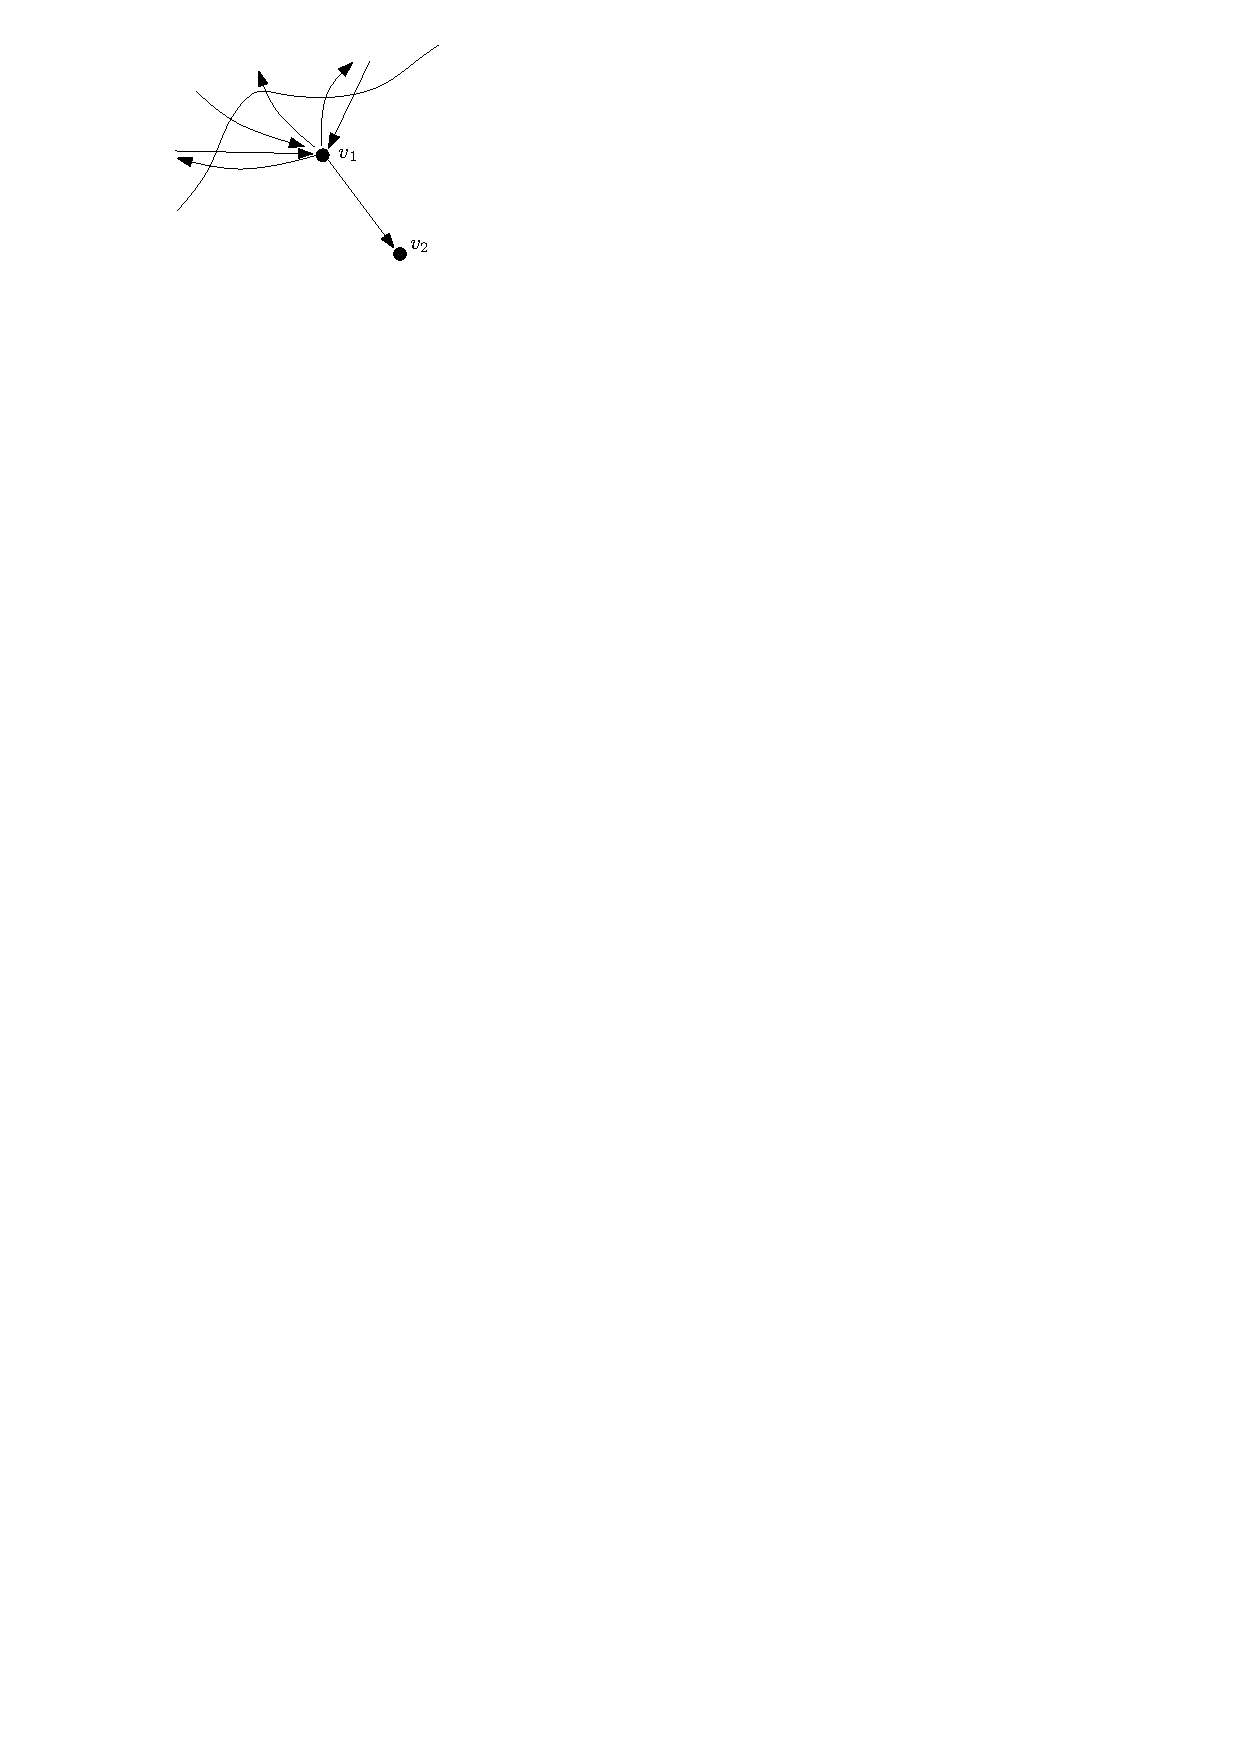
\includegraphics{pdf/dumbnode.pdf}
	}
\end{frame}

\begin{frame}{Algorithmus Rand-2Delta-Plus1}
	\begin{exampleblock}{Skizze}
	  \begin{itemize}[<+->]
			\item Hauptschleife
			\begin{itemize}
				\item Behalte die Farbe aus der letzten Runde (initial "`0"')
				\item Broadcaste aktuelle Farbe (Nachbarfarben dieser Runde $\rightarrow T$)
				\item Bei Konflikt 
				\begin{itemize}
					\item Mit Wahrscheinlichkeit $1/2$ wähle "`0"' als Farbe, sonst
					\item Wähle neue Farbe aus $[2\Delta+1] \backslash T$
				\end{itemize}
			\end{itemize}
		\end{itemize}
	\end{exampleblock}
\end{frame}

\begin{frame}{Beweisskizze}
	\begin{itemize}
		\item Gleiche Graph-Hierarchie
		\pause
		\item Statt terminiertem Knoten beweisen wir, dass Knoten "`stabil"' werden
		\pause
		\item Induktionsschritt weitestgehend gleich
		\pause
		\item Farben müssen erweitert werden, da alle Nachbarfarben als "`final"' angesehen werden
		\pause
		\item Laufzeit: $O(l \log n)$
	\end{itemize}
\end{frame}

\section{Untere Schranke}
\begin{frame}{Untere Schranke}
	\begin{itemize}[<+->]
		\item Für allgemeine Färbealgorithmen mit $O(\Delta)$ Farben:
		\item Deterministische Algorithmen haben untere Schranke $\Omega(l)$ (Kritischer Pfad)
		\item Randomisierte Algorithmen haben untere Schranke $\Omega(\min(l, \log n))$
		\item Beweisidee:
		\begin{itemize}
			\item Betrachte wie ein Konflikt propagiert
			\item<9> Konfliktwahrscheinlichkeit kann erst nach $\Omega(\log n)$ Schritten "`klein"' ($\leq 1-1/n^c, c>1$) sein
		\end{itemize}
	\end{itemize}
	\only<1-5>{
	\begin{figure}
	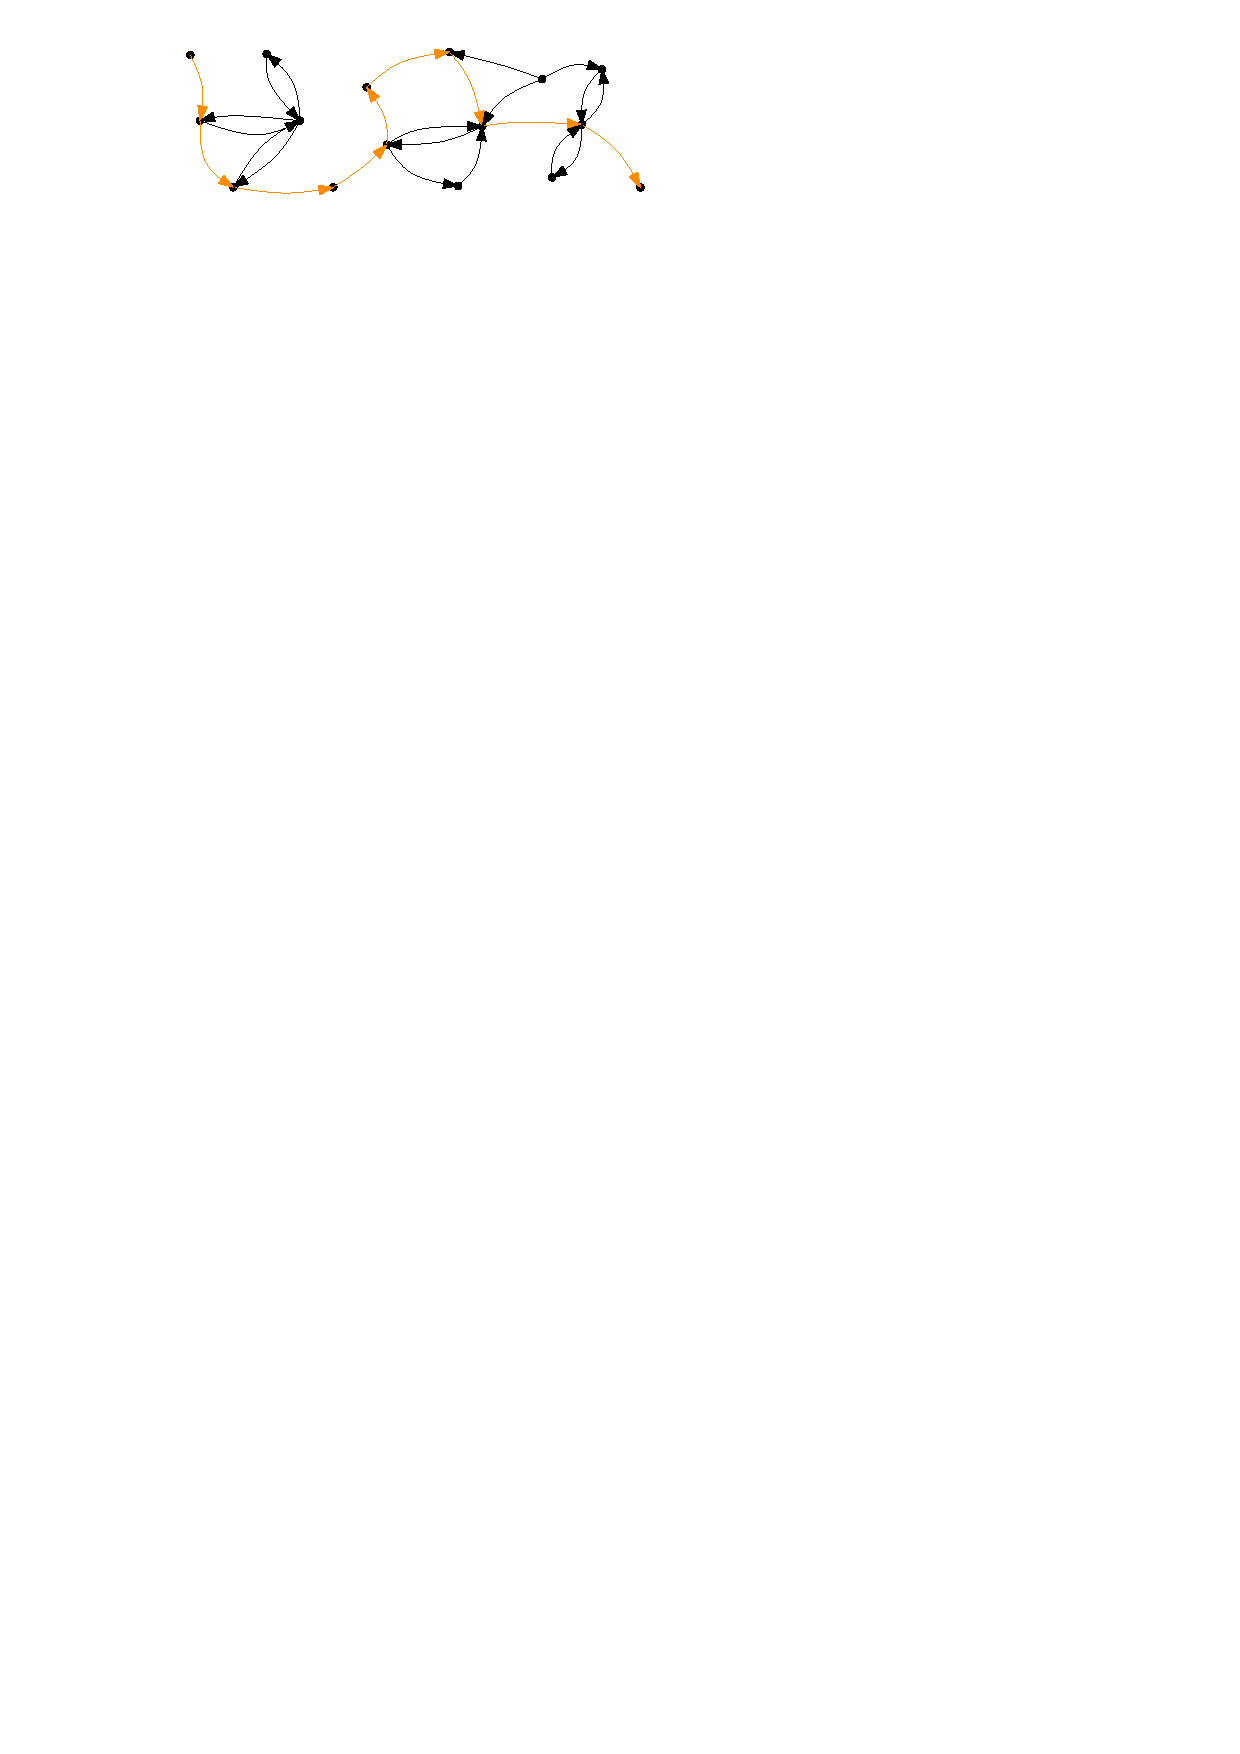
\includegraphics{pdf/longestpath.pdf}
	\end{figure}
	}
	\only<6>{
	\begin{figure}
	\includegraphics[page=2]{pdf/longestpath.pdf}
	\end{figure}
	}
	\only<7>{
	\begin{figure}
	\includegraphics[page=3]{pdf/longestpath.pdf}
	\end{figure}
	}
	\only<8,9>{
	\begin{figure}
	\includegraphics[page=4]{pdf/longestpath.pdf}
	\end{figure}
	}
\end{frame}

\section{Experiment}
\begin{frame}{Experiment}
	\begin{itemize}
		\item Simulation von Kommunikationsgraphen
		\item $100$ bis $10.000$ Knoten
		\item $X,Y \in [0,1]$
		\item Sendereichweiten pro Graphinstanz:
		\begin{itemize}
			\item Schnitt von $\frac{1}{200}$ bis $\frac{1}{5}$
			\item Maximale Abweichung von $\frac{3}{2}$ bis $8$
		\end{itemize}
		\item Über $50.000$ Simulationen
		\item Gleichverteilung von $n$ und den Sendereichweiten
		\end{itemize}
	\begin{figure}
	
	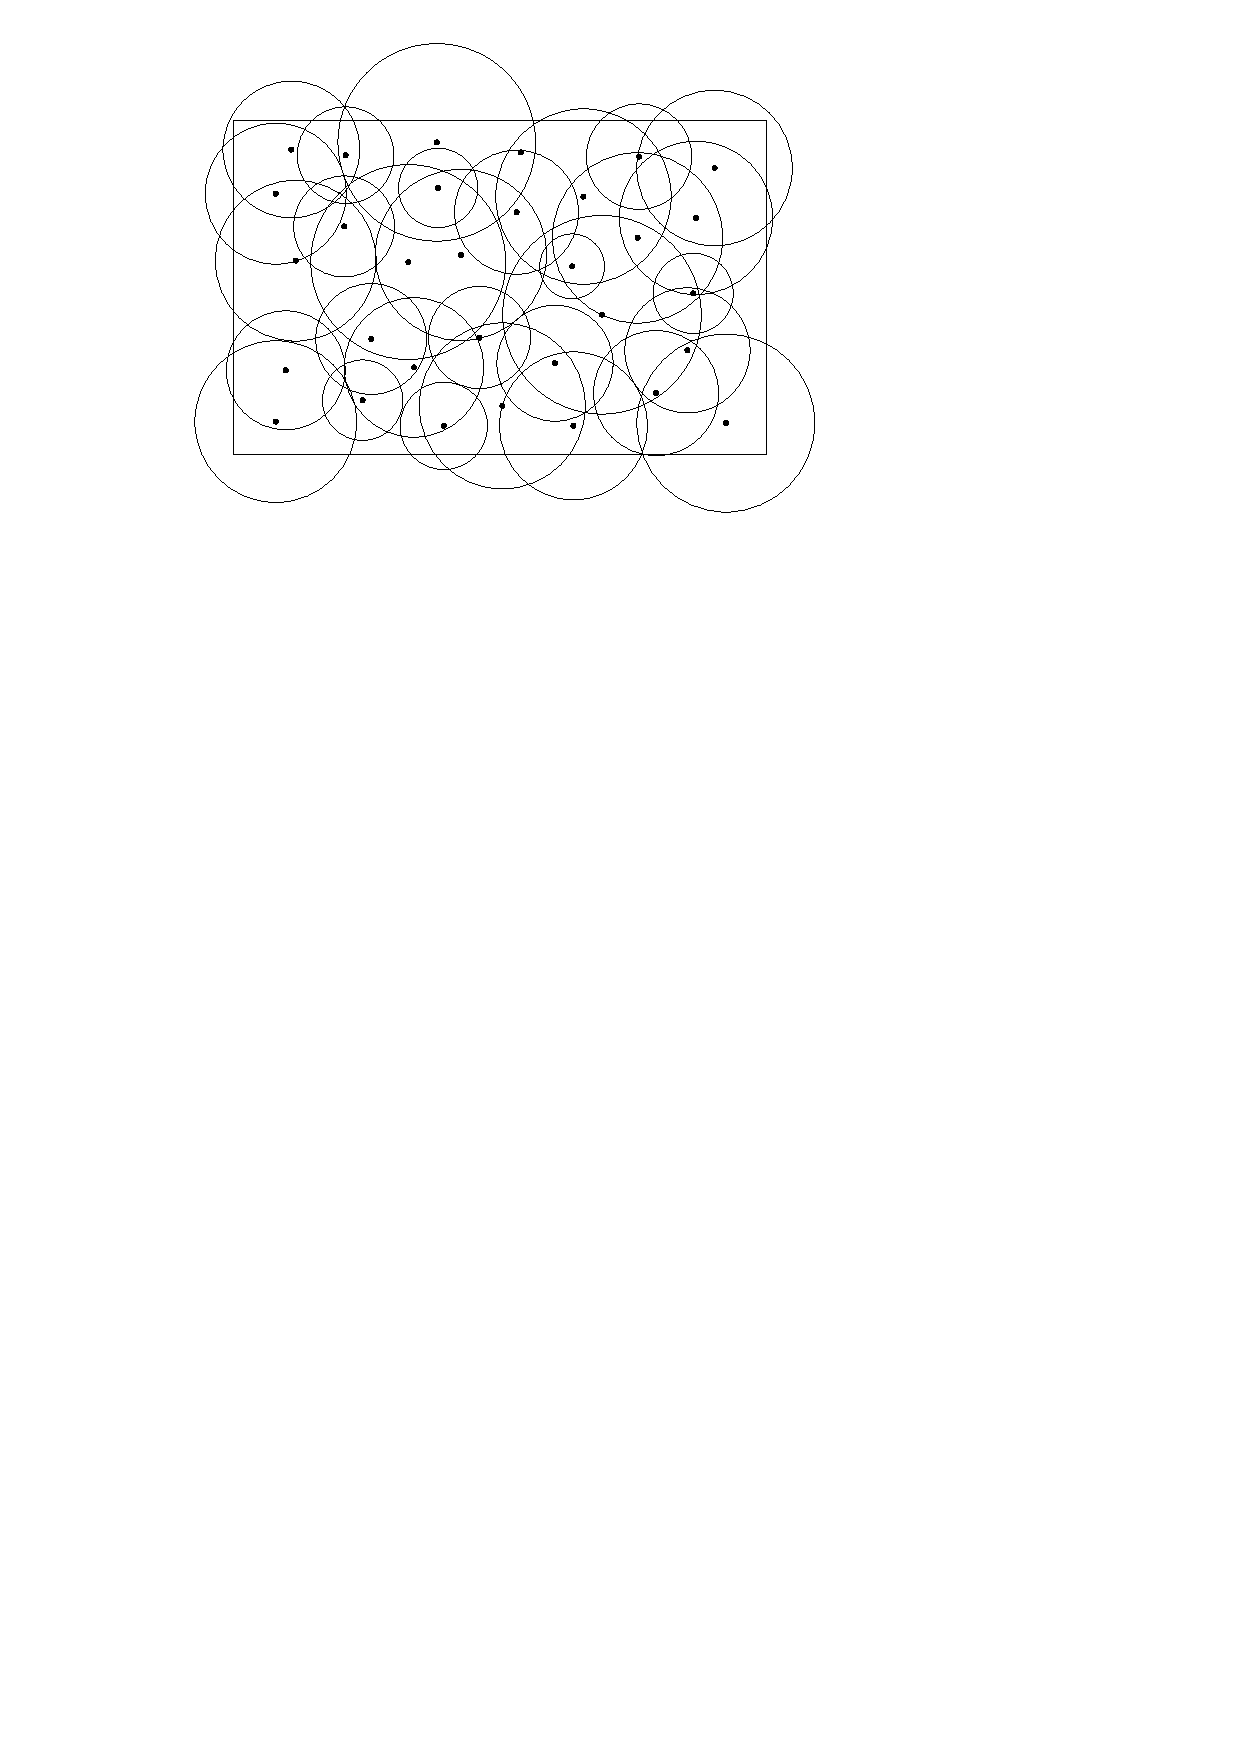
\includegraphics[width=5.5cm,clip=true,trim=19pt 29pt 24pt 38pt]{pdf/experiment.pdf}
	\end{figure}
	\end{frame}
	
	\begin{frame}{Interpretation der Daten}
	\begin{itemize}[<+->]
		\item $l$ steigt sublinear mit $n$ an
		\item Aber: $\Delta$ steigt linear mit $n$ an und $l$ steigt ebenfalls sublinear mit $\Delta$ an
		\item Mit festem $n$ verhält sich $l$ gegenüber $\Delta$ genauso wie mit allen $n$
		\item $\Rightarrow$ Abhängigkeit zu $n$ bedingt durch höheres $\Delta$
		\end{itemize}
		\includegraphics<1>[height=4cm]{pdf/boxplotnl.png}
		\includegraphics<2>[height=4cm]{pdf/boxplotndelta.png}
		\only<3>{
		\begin{tabular}{l l}
			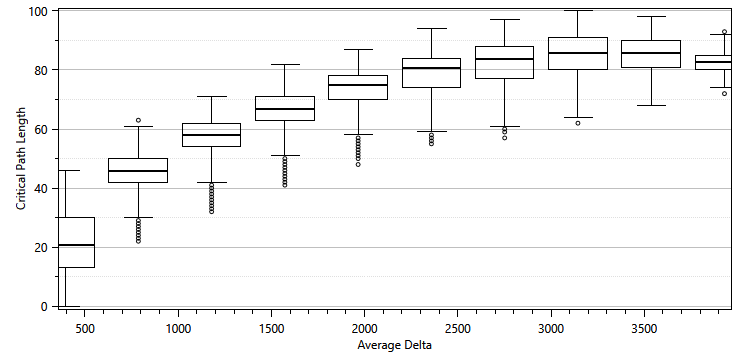
\includegraphics[height=2.5cm]{pdf/boxplotaveragedeltal.png}
			&
			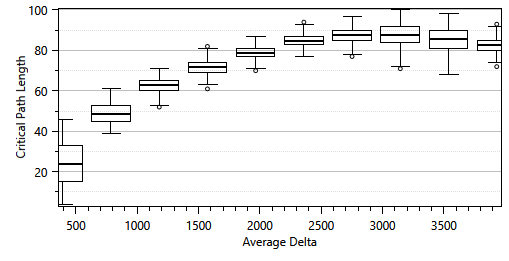
\includegraphics[height=2.5cm]{pdf/boxplotaveragedeltal8k.png}\\
			Plot über alle $n$
			&
			Plot über $n>8000$
		\end{tabular}
		}
\end{frame}

	\begin{frame}{Interpretation der Daten}
	\begin{itemize}[<+->]
		\item $l$ steigt mit der Sendereichweite (bis die Fläche abgedeckt ist)
		\item Eine höhere Sendereichweite bewirkt ebenfalls ein höheres $\Delta$
		\item Im Experiment bewirkt die höhere durchschnittliche Sendereichweite eine höhere Varianz
		\item Interpretation: $l$ steigt mit der Dichte des Graphen ($\Delta$) sowie der Varianz der Sendereichweiten
	\end{itemize}
	\center
	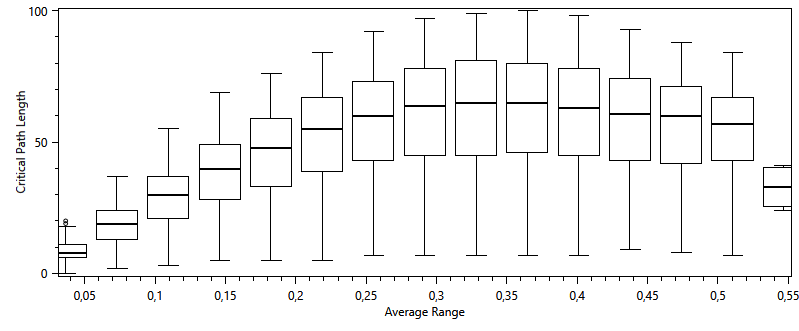
\includegraphics[height=4cm]{pdf/boxplotaveragerangel.png}	
\end{frame}

\section{Fazit}
\begin{frame}{Fazit}
	\begin{itemize}
		\item Algorithmen können unidirektionale Kanten ohne viel Komplexität berücksichtigen
		\pause
		\item Zwei Algorithmen vorgestellt: 
		\begin{itemize}
			\item $\Delta+1$ Färbung in $O(\Delta+l \log n)$ (mit Initialisierung) und
			\item $2\Delta+1$ Färbung in $O(l \log n)$
		\end{itemize}
		\pause
		\item Mit den vorgestellten Algorithmen können realitätsnahe Szenarien abgedeckt werden
		\pause
		\item Je größer die Sendereichweitenvarianz, um so größer wird $l$ und somit die erwartete Laufzeit
		\pause
		\item Ausblick: Differenz zwischen unteren Schranken und Laufzeiten verbessern
	\end{itemize}
\end{frame}


\end{document}
